\documentclass[aspectratio=169,10pt]{beamer}
\usetheme{metropolis}
\usepackage{amsmath,amssymb}
\usepackage{tikz}
\usetikzlibrary{positioning,arrows.meta,shapes.geometric,calc}
\usepackage{xcolor}
\usepackage{listings}

\definecolor{leangreen}{RGB}{34,139,34}
\definecolor{leanblue}{RGB}{70,130,180}
\definecolor{amber}{RGB}{255,191,0}

\lstdefinelanguage{Lean}{
  keywords={theorem, lemma, def, abbrev, variable, namespace, end, axiom, noncomputable},
  keywordstyle=\color{leanblue}\bfseries,
  comment=[l]{--},
  commentstyle=\color{gray}\itshape,
  string=[b]",
  stringstyle=\color{orange},
  basicstyle=\ttfamily\small,
  breaklines=true,
}

\title{\textbf{MPSLean}}
\subtitle{Formalizing the Fundamental Theorem of Matrix Product States in Lean 4}
\date{}
\author{}

\setbeamercolor{background canvas}{bg=black}
\setbeamercolor{normal text}{fg=white}
\setbeamercolor{title}{fg=white}
\setbeamercolor{frametitle}{fg=white,bg=black}
\setbeamercolor{block title}{fg=white,bg=gray!30!black}
\setbeamercolor{block body}{fg=white,bg=gray!10!black}

\begin{document}

\begin{frame}
\titlepage
\vspace{-2em}
\begin{center}
\huge\textcolor{leangreen}{\textbf{642 lines. 18 theorems. 0 axioms.}}

\vspace{1em}
\large Quantum many-body physics meets formal proof
\end{center}
\end{frame}

\begin{frame}{The Challenge}
\textbf{\LARGE When do $A$ and $B$ describe the same quantum physics?}

\vspace{0.5em}
\begin{columns}[T]
\column{0.55\textwidth}
\textbf{Matrix Product States:}
\[
|V^{(N)}\rangle = \sum_{i_1,\ldots,i_N} \mathrm{tr}(A^{i_1}\cdots A^{i_N}) |i_1\cdots i_N\rangle
\]

\vspace{0.5em}
\textbf{\textcolor{leangreen}{Fundamental Theorem:}}\\
Same MPV for all $N$ $\Leftrightarrow$ Gauge equivalence
\[
B^i = X A^i X^{-1}
\]

\vspace{0.3em}
\textbf{Our formalization:} Single-block case (injective tensors)

\column{0.45\textwidth}
\begin{center}
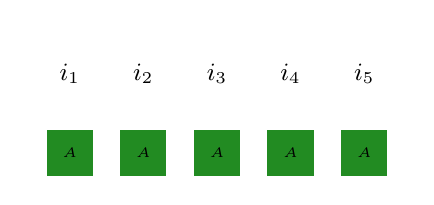
\begin{tikzpicture}[scale=0.85]
% Tensor nodes
\foreach \x in {1,2,3,4,5} {
  \node[rectangle,draw=white,fill=leangreen,minimum size=0.6cm] (A\x) at (\x*1.1,0) {\tiny $A$};
  % Physical leg pointing upward
  \draw[-,white,thick] (A\x.north) -- ++(0,0.4);
  \node[above=0.45cm of A\x] {\small $i_{\x}$};
}
% Virtual bonds (horizontal, bond dimension D)
\foreach \x in {1,2,3,4} {
  \pgfmathtruncatemacro{\next}{\x+1}
  \draw[-,white,thick] (A\x) -- (A\next);
}
% Trace boundary
\draw[-,white,thick,dashed] (A1.west) -- ++(-0.25,0);
\draw[-,white,thick,dashed] (A5.east) -- ++(0.25,0);
\node[above] at (3*1.1,1.3) {\textcolor{white}{\textbf{Tensor Network}}};
\end{tikzpicture}

\vspace{1.5em}
{\ttfamily\small
abbrev MPSTensor (d D : $\mathbb{N}$) :=\\ 
\hspace*{0.5em}Fin d $\to$ Matrix (Fin D) (Fin D) $\mathbb{C}$
}

\vspace{0.5em}
\textbf{Clean. Type-safe. Mathlib-powered.}
\end{center}
\end{columns}
\end{frame}

\begin{frame}{The Proof: 100\% Complete}
\vspace{-0.3em}
\begin{center}
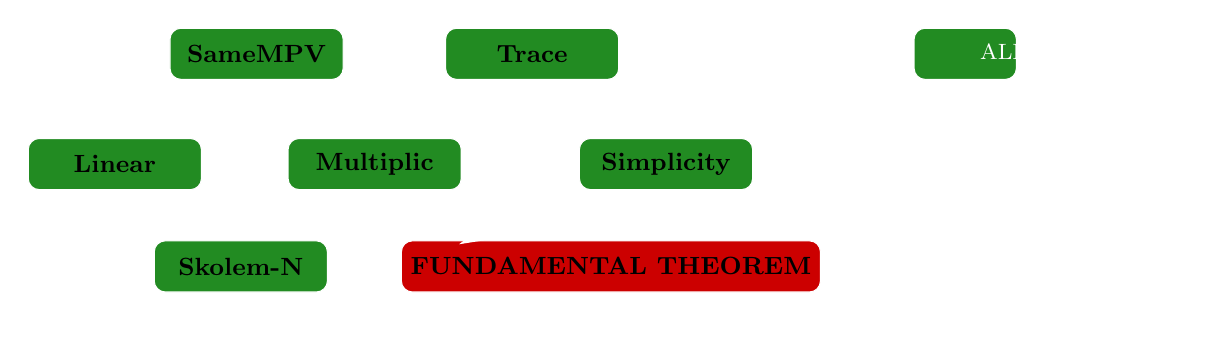
\begin{tikzpicture}[
  node distance=1.1cm and 0.7cm,
  lemma/.style={rectangle,draw=white,fill=leangreen,text=black,font=\small\bfseries,minimum width=2.2cm,minimum height=0.65cm,rounded corners},
  arrow/.style={-{Stealth[scale=1.3]},white,thick}
]

\node[lemma] (L2) at (0,3.2) {SameMPV};
\node[below=0.05cm of L2,font=\tiny,text=white] {traces agree};

\node[lemma] (L3) at (3.5,3.2) {Trace};
\node[below=0.05cm of L3,font=\tiny,text=white] {nondegen};

\node[lemma] (A1) at (-1.8,1.8) {Linear};
\node[below=0.05cm of A1,font=\tiny,text=white] {extension};

\node[lemma] (A2) at (1.5,1.8) {Multiplic};
\node[below=0.05cm of A2,font=\tiny,text=white] {ativity};

\node[lemma] (L5) at (5.2,1.8) {Simplicity};
\node[below=0.05cm of L5,font=\tiny,text=white] {bijective};

\node[lemma] (L6) at (-0.2,0.5) {Skolem-N};
\node[below=0.05cm of L6,font=\tiny,text=white] {via Mathlib};

\node[lemma,fill=red!80!black,minimum width=3.8cm] (MAIN) at (4.5,0.5) {\textbf{FUNDAMENTAL THEOREM}};
\node[below=0.05cm of MAIN,font=\tiny,text=white] {IsInjective and SameMPV implies GaugeEquiv};

\draw[arrow] (L2) -- (A2);
\draw[arrow] (A1) -- (MAIN);
\draw[arrow] (A2) -- (MAIN);
\draw[arrow] (L5) -- (MAIN);
\draw[arrow] (L6) -- (MAIN);
\draw[arrow] (L3) -- (A2);

\node[lemma,minimum width=1.3cm] at (9,3.2) {};
\node[text=white,font=\footnotesize] at (10.5,3.2) {ALL PROVED (18)};

\end{tikzpicture}
\end{center}

\vspace{0.3em}
\textbf{\Large Big Wins:}
\begin{itemize}
  \item[\textbf{\textcolor{leangreen}{$\checkmark$}}] \textbf{Skolem-Noether:} 84 lines via \texttt{AlgEquiv.eq\_linearEquivConjAlgEquiv}
  \item[\textbf{\textcolor{leangreen}{$\checkmark$}}] \textbf{Simplicity of $M_n(\mathbb{C})$:} Used \texttt{TwoSidedIdeal.ker}
  \item[\textbf{\textcolor{leangreen}{$\checkmark$}}] \textbf{Trace nondegeneracy:} 15 lines with single-entry matrices
  \item[\textbf{\textcolor{leangreen}{$\checkmark$}}] \textbf{Algebraic injectivity:} Bypassed Perron-Frobenius entirely!
\end{itemize}
\end{frame}

\begin{frame}{Roadmap: From Axioms to Applications}
\vspace{-0.3em}
\begin{center}
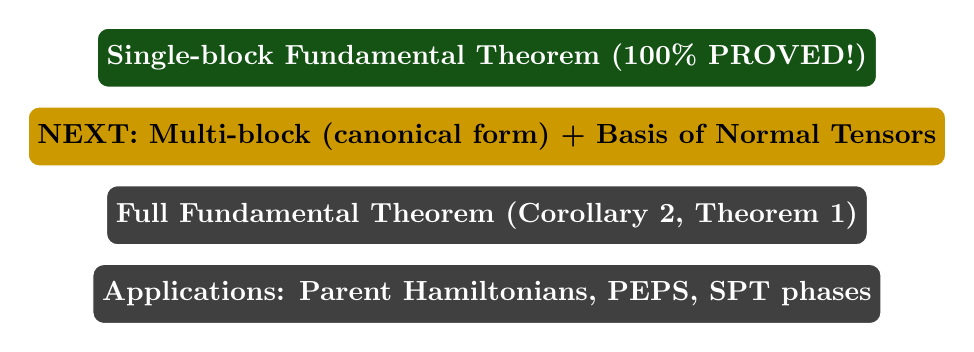
\begin{tikzpicture}[
  node distance=1.3cm,
  box/.style={rectangle,draw=white,text=white,font=\bfseries,minimum width=9.5cm,minimum height=0.75cm,rounded corners},
  done/.style={fill=leangreen!60!black},
  next/.style={fill=amber!80!black,text=black},
  future/.style={fill=gray!50!black}
]

\node[box,done] (current) at (0,3.6) {Single-block Fundamental Theorem (100\% PROVED!)};
\node[box,next] (axioms) at (0,2.6) {NEXT: Multi-block (canonical form) + Basis of Normal Tensors};
\node[box,future] (full) at (0,1.6) {Full Fundamental Theorem (Corollary 2, Theorem 1)};
\node[box,future] (app) at (0,0.6) {Applications: Parent Hamiltonians, PEPS, SPT phases};

\end{tikzpicture}
\end{center}

\vspace{0.8em}
\begin{columns}[T]
\column{0.48\textwidth}
\textbf{\Large The Numbers:}
\begin{itemize}
  \item \textbf{642 lines} of Lean 4
  \item \textbf{8 modules}, 18 theorems
  \item \textbf{0 axioms}, 0 sorries
  \item Mathlib v4.27.0
\end{itemize}

\column{0.48\textwidth}
\textbf{\Large The Vision:}
\begin{itemize}
  \item Formal quantum many-body theory
  \item Verified tensor network proofs
  \item Bridge to topological order
  \item Foundation for quantum algorithms
\end{itemize}
\end{columns}

\vspace{0.8em}
\begin{center}
\large\textbf{\textcolor{leangreen}{First complete formal proof of the Fundamental Theorem of MPS.}}
\end{center}
\end{frame}

\begin{frame}
\begin{center}
\Huge\textbf{\textcolor{leangreen}{MPSLean}}

\vspace{1em}
\Large Bridging quantum many-body physics\\and formal mathematics

\vspace{2em}
\LARGE\texttt{github.com/[your-repo]/MPSLean}

\vspace{1em}
\large Built on Mathlib v4.27.0\\
Lean 4 proving quantum information theory

\vspace{2em}
\textbf{\textcolor{leangreen}{The future is formally verified.}}
\end{center}
\end{frame}

\end{document}